\documentclass{scrartcl}
\usepackage[ansinew]{inputenc}
\usepackage[numbers,sort&compress]{natbib}
\usepackage{graphicx}
\usepackage{wrapfig}
\usepackage{subfig}
\usepackage{siunitx}
\usepackage{listings}
\lstset{%
	basicstyle=\footnotesize,	% the size of the fonts that are used for the code
	numbers=left,				% where to put the line-numbers
	stepnumber=2,				% the step between two line-numbers. If it's 1 each line will be numbered
	numbersep=7pt,				% how far the line-numbers are from the code
	frame=single,				% adds a frame around the code
	breaklines=true,			% break lines
	}
\usepackage{hyperref}

\title{How to perform a high resolution synchrotron radiation based x-ray tomographic microscopy wide field scan}
\subtitle{Or: how do I make a WF-SRXTM scan?}
\author{David Haberth�r}
\date{\today}

\newcommand{\imsize}{.618\linewidth}

\begin{document}

\maketitle

This document should give a walkthrough for successfully performing a high resolution synchrotron radiation based x-ray tomographic microscopy (SRXTM, \cite{Haberthuer2009d}) at TOMCAT, the beamline for TOmographic Microscopy and Coherent rAdiology experimenTs~\cite{Stampanoni2007}

\section{Setup of a WF-SRXTM scan}
After starting MATLAB on one of the computing consoles at TOMCAT (start it with entering \verb+matlab &+ in the console), open the file $\sim$\verb+/MATLAB/main.m+ in the home directory of our E-Account e11126 (\url{/sls/X02DA/data/e11126/}).

\begin{wrapfigure}{R}{0.25\linewidth}
	\centering
		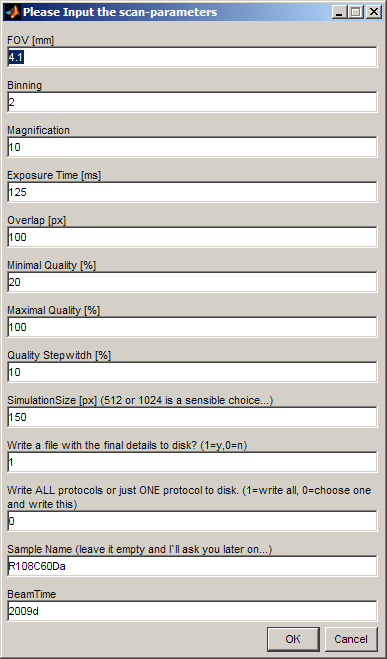
\includegraphics[width=\linewidth]{img/input}
	\caption{User dialog}
	\label{fig:user dialog}
\end{wrapfigure}

When you start this file, a user dialog asks you for the parameters for the scan (see figure~\ref{fig:user dialog}). You should have an idea about the diameter of your sample and some other parameters of your scan to be able to input those into this dialog and get an accurate simulation. Enter the desired field of view in the first line, the parameters of the setup like Binning, Magnification and Exposure Time on the second, third and fourth line.

The Overlap can be left around 100 px or changed to a value you'd like. The following three parameters (Minimal and Maximal Quality (Q\textsubscript{min}, Q\textsubscript{max}) as well as Quality Stepwidth (Q\textsubscript{step}) influecnce the calculation of the different protocols. Choose a broad range (like the defaults) for a good overview over the different possible protocols, choose a small range if <ou want to have a detailed choice over the different protocols.

The SimulationSize greatly influences the speed and accuracy of the calculation. If you enter a small size, the different protocols are calculated for a small Shepp--Logan pantom~\cite{Shepp1974} and the whole simulation is done quickly, but not very accurate. If you want to scan all multiple protocols between Q\textsubscript{min} and Q\textsubscript{max} and not only choose one of the protocols, you can safely leave this parameter on a small size, since the calculated number of Projections for each protocol does not depend on it. If you want to choose one protocol depending on the quality, you should set this parameter fairly high. This will increase the simulation time, but you'll get a more accurate estimation of the scanning quality.

The following fields are important for the writing of the parameter file, which are needed for in the next step, the acutal scan. If you want to write a preference file, put ``1'' in the 10\textsuperscript{th} field. This will generate a text file with the ``Sample Name'' you choose in the second to last field in the folder \url{/sls/X02DA/Data3/e11126/Beamtime}, where ``BeamTime'' is what you enter in the last field.

The MATLAB script will output several figures, some of them are shown in figure~\ref{fig:matlab}.
\renewcommand{\imsize}{.32\linewidth}%
\begin{figure}[htp]
	\centering
		\subfloat[Total Amount of Projections per Protocol]{%
			\label{subfig:totalamount}
			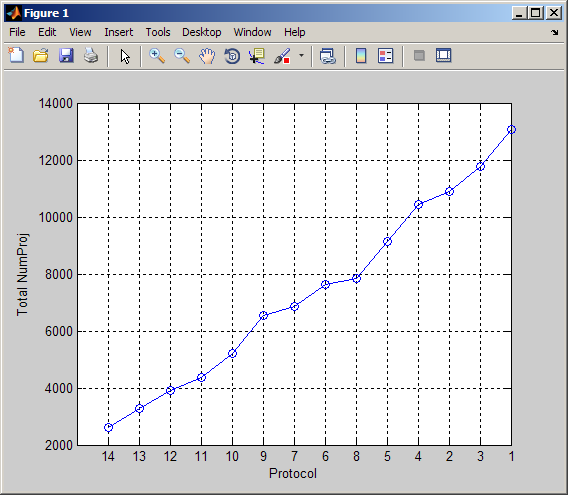
\includegraphics[width=\imsize]{img/fig01}%
			}\hfill%
		\subfloat[Error per pixel. x-axis shows the total amount of projections]{%
			\label{subfig:errorplot}
			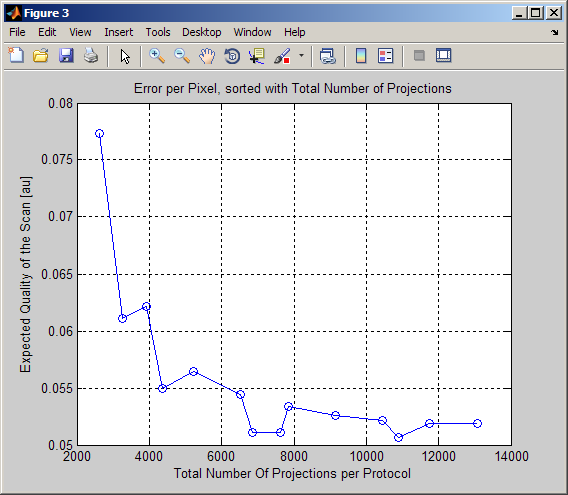
\includegraphics[width=\imsize]{img/fig03}%
			}\hfill%
		\subfloat[Quality of the scan plotted vs.\ scanning time needed (or vs.\ protocols)]{%
			\label{subfig:qualityplot}
			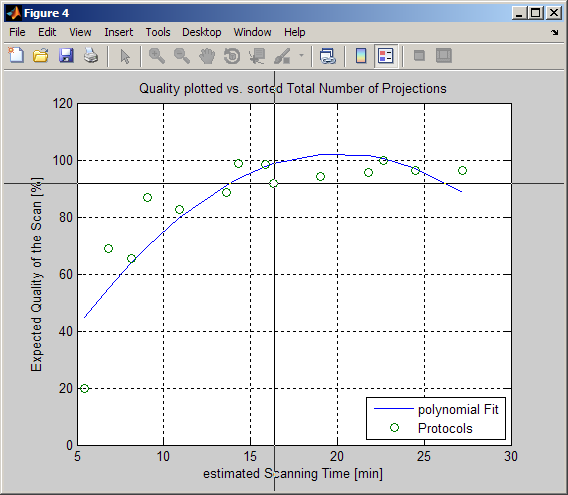
\includegraphics[width=\imsize]{img/fig04choosing}%
			}%		
	\caption{Output from main.m script. a) Total amount of projectiosn per protocol. This is the total amount of projections scanned for all subscans. b) Error of the difference image to the phantom compared to the total amount of projections. You can see a sharp increase in error for low amount of projections. c) Quality of the scan vs.\ scanning time, including a polynomial fit (only to guide the eye). The scanning time is estimates using the total amount of projections $\times$ the exposure time. This is where the user actually chooses a protocol (shown as cross at approx.\ \SI{16}{\minute} scanning time).}
	\label{fig:matlab}
\end{figure}

If you choose to scan only one protocol, you've entered ``0'' in the 11\textsuperscript{th} input field, the script asks you to choose one of the protocols in the qualityplot shown in figure~\ref{subfig:qualityplot} and then outputs a preference-file for one scan (see figures~\ref{subfig:choose1} and \ref{subfig:output1}). If you entered ``1'', you will not be asked to choose a protocol and the script outputs all possible protocols from Q\textsubscript{min} to $Q$\textsubscript{max} with a stepwidth of Q\textsubscript{step} to a preference file (see figure~\ref{subfig:outputall}). An example of a preference file for one protocol is shown in appendix~\ref{sec:preference file}.

\renewcommand{\imsize}{.5\linewidth}%
\begin{figure}[htp]%
	\centering
		\subfloat[Choose one protocol]{%
			\label{subfig:choose1}
			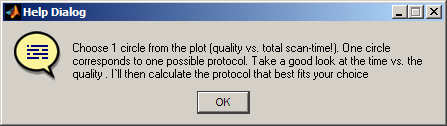
\includegraphics[width=\imsize]{img/chooseplot}%
			}%
		\subfloat[Output for one protocol]{%
			\label{subfig:output1}
			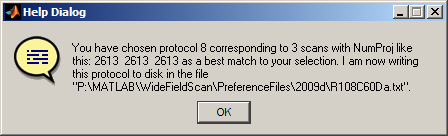
\includegraphics[width=\imsize]{img/chosenprotocol}%
			}\\%
		\subfloat[Output for all protocols]{%
			\label{subfig:outputall}
			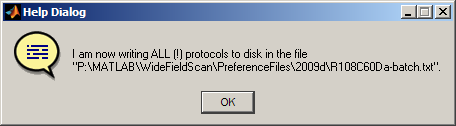
\includegraphics[width=\imsize]{img/writeall}%
			}
	\caption{Output Options}%
	\label{fig:options}%
\end{figure}

After you get this preference file, you can proceed to the next step.

\section{Scanning a sample with increased field of view}
To perform a wide field scan at TOMCAT, you need to adjust the sample in the beam, as you would do with a conventional scan. Make sure that you've aligned the sample in such a way that the feature you want to have in the center of the resulting wide field scan reconstructions is in the center of the preview window before proceeding (see the wiki-page: \url{http://www.ana.unibe.ch/~haberthuer/psi/perform_run} for a bit of details on how to align the sample). When you've aligned the sample, enter the ``SampleName'' into the corresponding field in the control panel of TOMCAT (on the machine with three screen). 

Copy \verb+widefieldscan_final.py+ from $\sim$\verb+/MATLAB/+ to the directory of the scan (\url{/sls/X02DA/Data3/e11126/Beamtime}). Start the Terminal of the machine next to the one with the three screens and ``cd'' to the directory of the BeamTime. Start the wide field scan with \verb+widefieldscan_fila.py PreferenceFile+ in the Terminal in the correct directory. ``PreferenceFile'' is the file that MATLAB has written after it has calculated all the protocols and you've selected one. If you've entered the parameters exactly like in figure~\ref{fig:user dialog}, the preference file you'll get is for one protocol and will be written to \url{/sls/X02DA/Data3/e11126/2009d/R108C60Da.txt}. 

When you've pressed Enter, the Python-script reads the SampleName from the EPICS-panel (you did set it correctly before, did you?), sets all other necessary parameters (Numer of projections, sample position, start and stop angle, etc.), waits for some seconds, and performs all necessary subscans with the correct amount of projections at the correct positions. The only thing you need to do is wait and maybe keep an eye on the console output, which informs you how things are progressing. The projections of all subscans are saved in the directories \url{/sls/X02DA/Data3/e11126/Beamtime/SampleName_si}), where s\textsubscript{i} is a directory for each of the three or five (or seven, but let's leave it below that) subscans.

\section{Stitching of the projections of the partial scans into merged pojections}
When the scan is finished, you have to stitch the projections of the several subscans to merged projections covering the chosen field of view. There's a MATLAB script in $\sim$\url{/MATLAB/MergeProjections/fct_mergeSubScansInterpolatedSelector.m} which performs such a merging.

This function needs ``AmountOfSubScans'', ``NumDarks'', ``NumFlats'', ``Tiff'', ``OutputSampleName'', ``OutputSuffix'' as input parameters and asks you to select the correct subscans to merge, performs the merging and writes the files to \url{/sls/X02DA/Data3/e11126/Beamtime/mrg/OutputSampleName-OutputSuffix-mrg}). 

The details of the parameters are:
\begin{description}
	\item [AmountOfSubScans] Amount of subscans which you've scanned to cover the field of view (s\textsubscript{1}--s\textsubscript{3} $\rightarrow$ 3 subscans)
	\item [NumDarks] The number of dark images you've acquired prior to the scan
	\item [NumFlats] The number of flat images you've acquired prior and after the scan. Both are needed to correct the projections. It's much easier to input them here than to parse them from the log-file, so I've chosen this way. If you don't know it, look at the log file of the firs subscan, and there you got everything.
	\item [Tiff] set this to ``1'' if you want .tif files as output. If you set it to ``0'', the script writes .DMP to disk (for historic reasons\ldots)
	\item [OutputSampleName] It might be necessary to restart a batch-scan after a beam dump, but you want to have all scans to have the same Name, so you can set this name here.
	\item [OutputSuffix] If you performed a batch scan of the same sample with different parameters, you can add an suffix to the Output, which then makes the protocols/parameters distinguishable in the output files.
\end{description}

If you've entered everything correctly, MATLAB first counts the files in the directories (again, much easier than logfile parsing), then reads the Darks and Flats to correct the projections. To set the correct gray values in the output files, MATLAB reads a subset of the projections of each subscan (the amount can be changed around line 160 of \verb+fct_mergeSubScansInterpolatedSelector.m+ in the variable \verb+GrayValueLoadHowMany+). Afterwards, the scripts calculates the Cutline using Chris' \verb+function_cutline.m+, merges the projections of the individual subscans together and writes a corrected and merged projection to the output path as described above. Additionally, MATLAB generates a faked logfile in the correct spot, and starts the generation of the sinograms with a call to \verb+sinooff_tomcat_j.py+ in the correct directory. Since the RecoManager (used for reconstruction) expects the (fake) .log-file in a certain spot, the script also hard-links the log-files.

The whole thing takes a while, so you can start the other scans while performing the merging. To be able to generate sinograms, you'll have to use MATLAB on 'x02da-cons-2', or else it won't work.

To be able to consistently perform the merging and choose a sane way of setting the OutputName I generally prefer to cobble together a little script which sets all parameters and calls the merging function, so I don't have to think too much. It's probably easiest if you open one of the old scripts (\verb+do_mergeSubScan2009c.m+) in MATLAB, adjust the parameters at the beginning, save it as a new file and then run this updated script, which calls the function with the correct parameters. With this you can easily keep track of which scans you've already merged.

\section{Reconstruting a WF-SRXTM scan}
\begin{enumerate}
	\item Sinogram: ok
	\item work on ``x02da-cons-2'' (perhaps via \verb+ssh+)
	\item check parameters with RecoManager (\verb+mozilla x02da-reco-1+ (oder so\ldots))
	\item DO NOT SUBMIT WITH RECOMANAGER
	\item 	\begin{lstlisting}
tif2rec_batch_web_grid_cn_david.py 3 20 /sls/X02DA/data/e11126/Data10/2009b/mrg/R108C36B-D-mrg/tif 1468.20 4,10,0.5 0 0,0,0,0 0,0.3,10 8,-0.025,0.35,0.0 "" 1,0,0 1
			\end{lstlisting}
	\item
\end{enumerate}


\bibliographystyle{unsrtnat}
\bibliography{references}

\clearpage

\appendix

\section{Appendix}
Explanation of the several involved files, for documentation and ``go on''-purpose. All necessary files to perform the steps mentioned above are under version control with  \href{http://en.wikipedia.org/wiki/Subversion_\%28software\%29}{subversion} at \url{http://code.ana.unibe.ch/} in the ``\href{http://code.ana.unibe.ch/websvn/listing.php?repname=wfs-sim&path=\%2F&sc=0}{wfs-sim}'' repository (the repository is called ``wfs-sim'', because it first contained only the files for the simulation. Now it included everything to perform a wide field scan).

Most of the files are functions which are called to perform several sub-tasks of the \verb+main.m+-file, and are denoted with a \verb+fct_+-prefix. A lot of files in the directory are used for testing the functions. Those testing files are denoted with a \verb+test_+-prefix.

\subsection{main.m}
\verb+main.m+ is the main MATLAB-File that is used for the simulation. The user is first asked for some input parameters like desired FOV (\verb+FOV_mm+), \verb+Binning+, \verb+Magnification+, Overlap between SubScans (\verb+Overlap_px+) and settings for the Quality (\verb+MinimalQuality+, \verb+MaximalQuality+ and \verb+QualityStepWidth+). From the Binning we can calculate the \verb+DetectorWith+, since the camera is 2048~	s wide and we assume that the full sensor is used. The \verb+pixelsize+ can be calculated from the Magnification, according to the table on the TOMCAT website. The DetectorWidth and the Overlap define the width of one segment (\verb+SegmentWidth_px+) and thus the \verb+AmountOfSubScans+. If the sample does not perfectly fit in the diameter of AmountOfSubScans $\times$ SegmentWidth, we're actually ``loosing`` imaging real estate, thus the user is informed of this. The actual FOV (\verb+ActualFOV_px+) is used for the calculation of the correct number of projections.

After we make sure that we have an odd amount of SubScans, we use the function \verb+fct_SegmentGenerator+ to calculate the \verb+NumberOfProjections+ from the inputs. The resulting table is $X$ amounts of SubScans wide and $Y$ protocols tall.

The user specifies the image size that should be used for the calculation of the simulated error (\verb+SimulationSize_px+). Since the radon and inverse radon transform is quite processor-intensive we simulate with a model where the images and reconstructions are of a smaller size. While making sure that the overlap for this model still stays above 5~pixels, we calculate the reduction factor according to the user input (\verb+ModelReductionFactor+) and scale the table with the number of projections, the phantom image (\verb+ModelImage+) and the detector width (\verb+ModelDetectorWidth+) with this reduction factor. After we have calculated a full size sinogram and a full size reconstruction (\verb+ModelMaximalSinogram+ and \verb+ModelMaximalReconstruction+), we use the function \verb+fct_ErrorCalculation+ for details on this function) to calculate the error of each protocol.

This error is kept track of in \verb+AbsoluteError+ and \verb+ErrorPerPixel(Protocol)+, once as absolute and once normalized to the total amount of pixels in the image. After we've sorted the number of projections and summed the amount of projections for each protocol (\verb+TotalSubScans+), we plot this value versus the \verb+QualityMeasure+. The Quality is calculated in such a way that we subtract the maximum of the Error per Pixel from all the Errors per Pixel, so we get a high value for low Errors and vice versa. After we've scaled this value to the minimal and maximal quality the user has input, we provide the user a mean of choosing the protocol, that suits his needs in terms of quality and scanning time.

The chosen value is saved into \verb+User_NumProj+ and subsequently written to disk to a file \verb+UserSampleName+.txt which contains the details of the chosen Protocol, including \verb+InBeamPosition+ and the angles of the rotation stage (which are currently hardcoded as \verb+RotationStartAngle+=46� and \verb+RotationStopAngle+=225�).

\subsection{fct\_ErrorCalculation.m}
This function uses the model phantom, the number of projections of each subscan and the maximal reconstruction as an input. Inside the function we split the image into different parts (no overlap is calculated!) for each subscan. According to the different amount of subscans from the outer to the inner scans we interpolate rows of these parts from the sinogram of the maximal image using another function (\verb+fct_InterpolateImage+). This corresponds to a different amount of recorded projections, since these are ``encoded'' in the rows of the sinogram. Since MATLAB calculates the sinogram 90� rotated to what we know and like, the sinogram is internally flipped (thus we get the ``interpolating in horizontal direction'' when the numbers of projections for the scans need to be interpolated.

The resulting reconstruction from the correctly interpolated sinogram is shown in together with the difference image. An error-measure is then calculated from this image in such a way that we take the sum over each pixel --- in MATLAB written as 
$\sum_{horiz.}(\sum_{vert.} ( \textrm{DiffImg} ) )$
---  of the difference image of the resulting reconstruction and the model image. 
The difference image is calculated with the MATLAB-function \verb+imabsdiff+ which calculates the absolute difference between two images, so we don't have to take the square of this error.

\section{fct\_InterpolateImage.m}
This function came from my lack of memorization of the correct interpolation syntax. It takes an image as input, wants to know how many lines should be interpolated over (interpolate every $x^{th}$ line and spits out the interpolated image. An optional parameter decides if it should interpolate horizontally or vertically (needed since MATLAB makes the sinograms 90� rotated to what we like and know\ldots).

\section{fct\_SegmentGenerator.m}
This function takes the sample width (\verb+ActualFOV_px+), the amount of SubScans and the quality details as input. The fundamental number of projections $N$ is calculated as $N= \textrm{FOV} * \frac{\pi}{2}$ which is according to the normally recorded 1500~projections for a detector size of 1024~pixels.

Afterwards a table with the number of projections for each segment/subscan is generated. If the quality ranges from 10--100\% in 10\% steps we have 10 protocols. Since we want to have a reduction in time, we now divide the inner protocols with 2, 4, 6, 8 and 10. This also works if we have not three, but five or seven subscans. All the protocols where the sampling rate is lower than 30\% are discarded (but only if the minimal quality specified by the user ain't lower than that\ldots).

In the end we get a table with $X$ colums and $Y$ rows, where $X$ is the amount of subscans and $Y$ are the different protocols.

\section{Example of a preference file}%
\label{sec:preference file}
Below is an example of a preference file which is generated by the \verb+main.m+-MATLAB file and contains all parameters for one wide field scan. Such a .txt-file is then subsequently read by the \verb+widefieldscan_final.py+-file and used to set the parameters in the EPICS-panel at TOMCAT.

\lstinputlisting{PreferenceFile.txt}

\end{document}